\documentclass[11pt]{article}
\usepackage{amssymb}
\usepackage{amsthm}
\usepackage{enumitem}
\usepackage{amsmath, physics}
\usepackage{bm}
\usepackage{adjustbox}
\usepackage{mathrsfs}
\usepackage{graphicx}
\usepackage{siunitx}
\usepackage[mathscr]{euscript}

\title{\textbf{Solved selected problems of Classical Electrodynamics - Hans Ohanian}}
\author{Franco Zacco}
\date{}

\addtolength{\topmargin}{-3cm}
\addtolength{\textheight}{3cm}

\newcommand{\N}{\mathbb{N}}
\newcommand{\Z}{\mathbb{Z}}
\newcommand{\Q}{\mathbb{Q}}
\newcommand{\R}{\mathbb{R}}
\newcommand{\diam}{\text{diam}}
\newcommand{\cl}{\text{cl}}
\newcommand{\bdry}{\text{bdry}}
\newcommand{\inter}{\text{int}}
\newcommand{\uvi}{\bm{i}}
\newcommand{\uvj}{\bm{j}}
\newcommand{\uvk}{\bm{k}}
\newcommand{\hatx}{\bm{\hat{x}}}
\newcommand{\haty}{\bm{\hat{y}}}
\newcommand{\hatz}{\bm{\hat{z}}}
\newcommand{\hatrho}{\bm{\hat{\rho}}}
\newcommand{\hatphi}{\bm{\hat{\phi}}}
\newcommand{\hatr}{\bm{\hat{r}}}
\newcommand{\hatn}{\bm{\hat{n}}}
\newcommand{\hattheta}{\bm{\hat{\theta}}}
\newcommand{\sci}[1]{\times 10^{#1}}
\newcommand\numberthis{\addtocounter{equation}{1}\tag{\theequation}}

\theoremstyle{definition}
\newtheorem*{solution*}{Solution}
\renewcommand*{\proofname}{\bf{Solution}}

\begin{document}
\maketitle
\thispagestyle{empty}

\section*{Chapter 5 - Electric Energy}

\subsection*{Problems}
\begin{proof}{\textbf{1.}}
Following the same logic we used to compute the electrostatic potential energy
$U$ for two charges at a distance $r$ and ignoring the self-energy of each
charge we see that $U$ in this case must be
\begin{align*}
    U = \frac{q_1 q_2}{r} + \frac{q_1 q_3}{r} + \frac{q_1 q_4}{r} +
    \frac{q_2 q_3}{r} + \frac{q_2 q_4}{r} + \frac{q_3 q_4}{r}
\end{align*}
Where $r$ is the distance of one particle from another particle, and since we
are dealing with a tetrahedron, then all distances are the same.
Therefore, since $r = 3 \times 10^{-13} ~cm$ and
$q_i = +2e = 9.606\times 10^{-10}~esu$ then
\begin{align*}
    U = 6 \cdot \frac{9.606\times 10^{-10} \cdot 9.606\times 10^{-10}~esu^2}
    {3 \times 10^{-13} ~cm}
    = 1.845 \times 10^{-5} ~erg
\end{align*}
\end{proof}

\cleardoublepage
\begin{proof}{\textbf{2.}}\\
Let us consider a system of two identical thin rods of plastic of length $L$
each carrying a charge $Q$ distributed uniformly along their length.
The rods are aligned, with a distance $d$ between their nearest ends.
\\
Let us consider two infinitesimal pieces of each rod where each one contains
a charge $dq = Qdx/L$ then we can compute the potential energy between them as
\begin{align*}
    dU = \frac{dq dq'}{d + x  + x'} = \frac{Q^2 dx dx'}{L^2(d + x  + x')}
\end{align*}
Where $x$ and $x'$ are the distances to the infinitesimal pieces measured from
the nearest ends. Then by integration we have that
\begin{align*}
    U &= \frac{Q^2}{L^2}\int_0^L \int_0^L \frac{dx dx'}{d + x  + x'}\\
    &= \frac{Q^2}{L^2}\int_0^L \bigg[\log(d + x + x')\bigg]_0^L dx'\\
    &= \frac{Q^2}{L^2}\int_0^L \bigg[\log(d + L + x') - \log(d + x')\bigg] dx'\\
    &= \frac{Q^2}{L^2}
    \bigg[(d + L + x')\log(d + L + x') - x'\bigg]_0^L
    - \bigg[(d + x')\log(d + x') - x'\bigg]_0^L\\
    &= \frac{Q^2}{L^2}
    \bigg[(d + 2L)\log(d + 2L) - 2(d + L)\log(d + L) + d\log(d)\bigg]\\
    &= \frac{Q^2}{L^2}
    \bigg[(d + 2L)(\log(d + 2L) - \log(d + L)) - d(\log(d + L) - \log(d))\bigg]\\
    &= \frac{Q^2}{L^2}
    \bigg[(d + 2L)\log(\frac{d + 2L}{d + L}) - d\log(\frac{d + L}{d})\bigg]
\end{align*}
Finally, we can compute the repulsive force between the rods by differentiation
of $U$ with respect to $d$ as follows
\begin{align*}
    F &= \pdv{U}{d}\\
    &= \frac{Q^2}{L^2}\bigg[
        \log(\frac{d + 2L}{d + L}) - \frac{L}{L + d}
        - \log(\frac{d + L}{d}) + \frac{L}{L + d}
    \bigg]\\
    &= \frac{Q^2}{L^2}\bigg[
        \log(\frac{d + 2L}{d + L}) - \log(\frac{d + L}{d})
    \bigg]\\
    &= \frac{Q^2}{L^2}\bigg[
        \log(1 + \frac{L}{d + L}) - \log(1 + \frac{L}{d})
    \bigg]
\end{align*}
Where we used that
$$\frac{d + 2L}{d + L} = \frac{d + L + L}{d + L}
= \frac{d + L}{d + L} + \frac{L}{d + L} = 1 + \frac{L}{d + L}$$
\end{proof}

\cleardoublepage
\begin{proof}{\textbf{4.}}\\
Let us consider a charge distribution with spherical symmetry and a charge
density $\rho(r) = kr^{-n}$, where $k$ and $n$ are positive constants and
$0 \leq r < R$.
\\
Let us compute the electric field $E$ by using Gauss law as follows
\begin{align*}
    \int_0^{2\pi}\int_0^\pi E ~r^2 \sin\theta d\theta d\phi
    &= 4\pi \int_0^r \int_0^{2\pi}\int_0^\pi
    \rho(r)~r^2\sin\theta d\theta d\phi dr\\
    4\pi E r^2 &= (4\pi)^2 k \int_0^r r^{2-n}~ dr\\
    E &= \frac{4\pi k}{r^2} \bigg[\frac{r^{3-n}}{3-n}\bigg]_0^r\\
    E &= \frac{4\pi k}{r^2} \frac{r^{3-n}}{3-n}\\
    E &= \frac{4\pi k}{3 -n} r^{1-n}
\end{align*}
Where must be that $n < 3$ otherwise the integral diverges.
Also, we used that $E$ is spherically symmetric.
\\
Now, we can compute the electrostatic potential energy using equation (9)
as follows
\begin{align*}
    U &= \frac{1}{8\pi}\int E^2~dV\\
    &= \frac{1}{8\pi}\int_0^R \int_0^{2\pi}\int_0^\pi
    E^2~r^2\sin\theta d\theta d\phi dr\\
    &= \frac{1}{8\pi}\int_0^R \int_0^{2\pi}\int_0^\pi
    \bigg(\frac{4\pi k}{3 -n} r^{1-n}\bigg)^2~r^2\sin\theta d\theta d\phi dr\\
    &= \frac{1}{8\pi}\bigg(\frac{4\pi k}{3 - n}\bigg)^2
    \int_0^R \int_0^{2\pi}\int_0^\pi
    r^{4-2n}~\sin\theta d\theta d\phi dr\\
    &= \frac{4\pi}{8\pi}\bigg(\frac{4\pi k}{3 - n}\bigg)^2 \int_0^R
    r^{4-2n}~dr\\
    &= \frac{1}{2}\bigg(\frac{4\pi k}{3 - n}\bigg)^2 
    \bigg[\frac{r^{5-2n}}{5-2n}\bigg]_0^R\\
    &= \frac{1}{2}\bigg(\frac{4\pi k}{3 - n}\bigg)^2\frac{R^{5-2n}}{5-2n}
\end{align*}
Must be that $5 - 2n > 0$ otherwise the integral diverges, so must be that
\begin{align*}
    n < \frac{5}{2}
\end{align*}
\end{proof}

\cleardoublepage
\begin{proof}{\textbf{5.}}\\
Let the charge density of the proton be $\rho = (e/8\pi a^3) e^{-r/a}$, then,
we can compute the electric field $E$ by taking a spherical Gaussian surface
around the proton. So using that $E$ is spherically symmetric, we have that
\begin{align*}
    \int_0^{2\pi}\int_0^\pi E ~r^2 \sin\theta d\theta d\phi
    &= 4\pi \int_0^r \int_0^{2\pi}\int_0^\pi
    \rho(r)~r^2\sin\theta d\theta d\phi dr\\
    4\pi E r^2 &= \frac{(4\pi)^2 e}{8\pi a^3} \int_0^r r^2 e^{-r/a}~ dr\\
    4\pi E r^2 &= \frac{2\pi e}{a^3}\bigg[
        -r^2a e^{-r/a}\bigg|_{0}^r  + 2a\int_{0}^r re^{-r/a}~dr
    \bigg]\\
    E &= \frac{e}{2a^3r^2}\bigg[
        -r^2a e^{-r/a}  + 2a\bigg[-are^{-r/a}\bigg|_{0}^r + a\int_{0}^r e^{-r/a}~dr\bigg]
    \bigg]\\
    E &= \frac{e}{2a^3r^2}\bigg[
        -r^2a e^{-r/a} - 2a^2re^{-r/a} + 2a^3 - 2a^3e^{-r/a}
    \bigg]\\
    E &= \frac{e}{2a^3r^2}\bigg[2a^3 - ae^{-r/a}(r^2 + 2ar + 2a^2)\bigg]\\
    E &= \frac{e}{r^2}
    \bigg[1 - e^{-r/a}\bigg(1 + \frac{r}{a} + \frac{r^2}{2a^2}\bigg)\bigg]
\end{align*}
Where we used integration by parts twice.
\\
If we let $x = r/a$ then the equation becomes
\begin{align*}
    E &= \frac{e}{x^2a^2}
    \bigg[1 - e^{-x}\bigg(1 + x + \frac{x^2}{2}\bigg)\bigg]
\end{align*}
Plotting this equation gives us
\begin{center}
    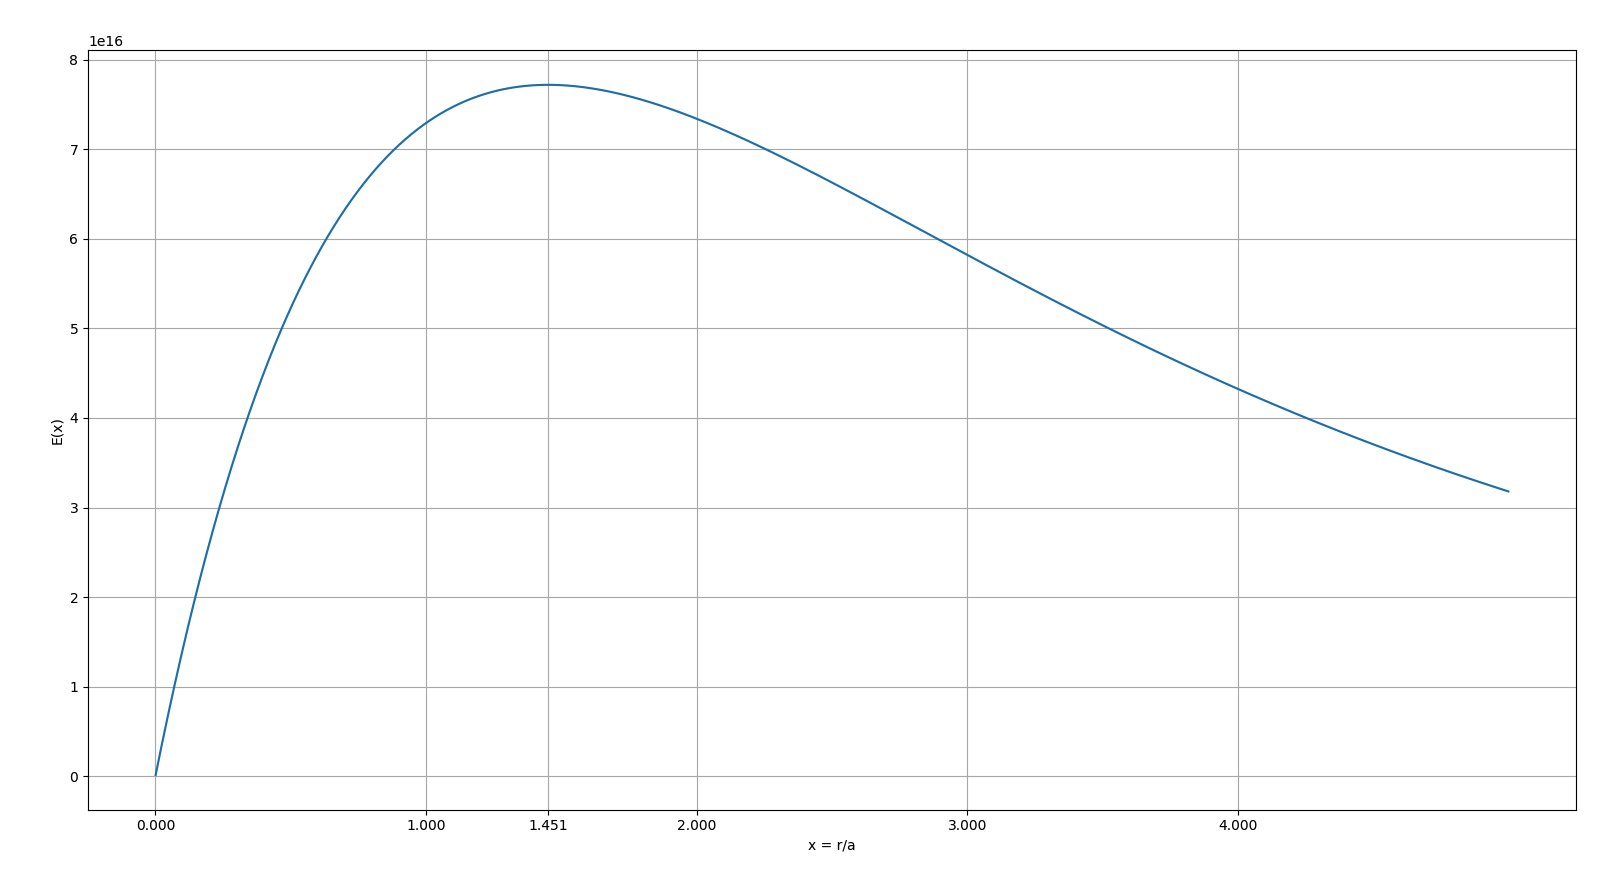
\includegraphics[scale=0.25]{ch5-5.png}
\end{center}
From which we see that the maximum $E$ happens at $x \approx 1.451$ and hence
$r = 3.337\times 10^{-14}~cm$.
\\
To find the net electrostatic self-energy we need to compute
\begin{align*}
    U = \frac{1}{8\pi} \int E^2~dV
\end{align*}
Then
\begin{align*}
    U &= \frac{1}{8\pi}\int_0^\infty \int_0^{2\pi}\int_0^\pi \frac{e^2}{r^4}
    \bigg[1 - e^{-r/a}\bigg(1 + \frac{r}{a} + \frac{r^2}{2a^2}\bigg)\bigg]^2
    ~r^2\sin\theta d\theta d\phi dr\\
    U &= \frac{e^2}{2}\int_0^\infty \frac{1}{r^2}
    \bigg[1 - e^{-r/a}\bigg(1 + \frac{r}{a} + \frac{r^2}{2a^2}\bigg)\bigg]^2
    ~dr
\end{align*}
If we let $u = r/a$ then $du = dr/a$, so, we get that
\begin{align*}
    U &= \frac{e^2}{2a}\int_0^\infty \frac{1}{u^2}
    \bigg[1 - e^{-u}\bigg(1 + u + \frac{u^2}{2}\bigg)\bigg]^2 ~du
\end{align*}
Where solving this integral numerically we get that
\begin{align*}
    U &= \frac{e^2}{2a}\frac{5}{16} = 1.567\times 10^{-6}~erg = 0.978~MeV
\end{align*}
The value of the rest-mass energy of the proton is $938.27~MeV$.
\end{proof}

\cleardoublepage
\begin{proof}{\textbf{7.}}\\
Let us consider a sphere of radius $R_{in}$ with a charge $+e$ uniformly
distributed, and a concentric shell of inner radius $R_{in}$ and outer radius
$R_{ex}$ with a charge $-e$ uniformly distributed.
\\
Let us consider first the sphere alone, we know that the electric field in this
case is
\begin{align*}
    \bm{E}_{sph} &= +\frac{er}{R_{in}^3} \hatr \qquad r \leq R_{in}\\
    \bm{E}_{sph} &= +\frac{e}{r^2} \hatr \qquad r \geq R_{in}
\end{align*}
On the other hand, for the shell alone we have that
\begin{align*}
    \bm{E}_{she} &= 0 \qquad r < R_{in}
\end{align*}
Because there is no charge enclosed.
\\
To determine the electric field when $R_{in} < r < R_{ex}$ we consider a
Gaussian surface to be a surface of a sphere with radius 
$R_{in} < r < R_{ex}$ then by Gauss' law we have that
\begin{align*}
    \int E_{she}\cdot dS = 4\pi E_{she} r^2
\end{align*}
Since the Gaussian surface we are taking, encloses a radius smaller than
$R_{ex}$ then the charge enclosed is
\begin{align*}
    Q &= V \rho\\
    &= \bigg[\frac{4}{3}\pi r^3 - \frac{4}{3}\pi R_{in}^3\bigg]
    \frac{-e}{\frac{4}{3}\pi R_{ex}^3 - \frac{4}{3}\pi R_{in}^3}\\
    &= \frac{-e(r^3 - R_{in}^3)}{R_{ex}^3 - R_{in}^3}
\end{align*}
Then the electric field is
\begin{align*}
    4\pi E_{she} r^2 = 4\pi\frac{-e(r^3 - R_{in}^3)}{R_{ex}^3 - R_{in}^3}\\
    \bm{E}_{she} = \frac{-e}{R_{ex}^3 - R_{in}^3}\bigg(r - \frac{R_{in}^3}{r^2}\bigg)\hatr
\end{align*}
Now, if $r \geq R_{ex}$ the shell looks like an sphere to an external Gaussian
surface so the electric field is
\begin{align*}
    \bm{E}_{she} &= -\frac{e}{r^2} \hatr \qquad r \geq R_{ex}
\end{align*}
So using the superposition principle we can compute the total electric field,
hence if $r \leq R_{in}$ we get that
\begin{align*}
    \bm{E} &= +\frac{er}{R_{in}^3}\hatr + 0
    = +\frac{er}{R_{in}^3}\hatr
\end{align*}
If $R_{in} < r < R_{ex}$
\begin{align*}
    \bm{E} &= +\frac{e}{r^2}
    - \frac{e}{R_{ex}^3 - R_{in}^3}\bigg(r - \frac{R_{in}^3}{r^2}\bigg)~\hatr\\
    &= +\frac{e}{r^2}
    - \frac{er}{R_{ex}^3 - R_{in}^3}
    + \frac{eR_{in}^3}{r^2(R_{ex}^3 - R_{in}^3)}~\hatr\\
    &= \frac{e}{r^2}\bigg(1 + \frac{R_{in}^3}{R_{ex}^3 - R_{in}^3}\bigg)
    - \frac{er}{R_{ex}^3 - R_{in}^3}~\hatr
\end{align*}
And if $r \geq R_{ex}$
\begin{align*}
    \bm{E} &= +\frac{e}{r^2}\hatr + \frac{-e}{r^2}\hatr = 0
\end{align*}
With this results we can compute the energy density $T^{00}$ as follows
\begin{align*}
    T^{00} &= \frac{e^2r^2}{8\pi R_{in}^6} &r \leq R_{in}\\
    T^{00} &= \frac{1}{8\pi}
    \bigg[\frac{e}{r^2}\bigg(1 + \frac{R_{in}^3}{R_{ex}^3 - R_{in}^3}\bigg)
    - \frac{er}{R_{ex}^3 - R_{in}^3}\bigg]^2 &R_{in} < r < R_{ex}\\
    T^{00} &= 0 &r \geq R_{ex}
\end{align*}
To determine the electrostatic energy we integrate the energy density.
For $r \leq R_{in}$ we have that 
\begin{align*}
    U &= \int T^{00}~dV\\
    &= 4\pi \int_{0}^{R_{in}}\frac{e^2r^2}{8\pi R_{in}^6} r^2~dr\\
    &= \frac{e^2}{2R_{in}^6} \int_{0}^{R_{in}} r^4~dr\\
    &= \frac{e^2}{2R_{in}^6} \bigg[\frac{R_{in}^5}{5}\bigg]\\
    &= \frac{e^2}{10R_{in}}
\end{align*}
For $R_{in} < r < R_{ex}$
\begin{align*}
    U &= \frac{4\pi}{8\pi}\int_{R_{in}}^{R_{ex}}
    \bigg[\frac{e}{r^2}\bigg(1 + \frac{R_{in}^3}{R_{ex}^3 - R_{in}^3}\bigg)
    - \frac{er}{R_{ex}^3 - R_{in}^3}\bigg]^2 r^2~dr\\
    &= \frac{1}{2}\int_{R_{in}}^{R_{ex}}
    \frac{e^2}{r^2}\bigg(1 + \frac{R_{in}^3}{R_{ex}^3 - R_{in}^3}\bigg)^2
    - 2e^2r\bigg(\frac{1}{R_{ex}^3 - R_{in}^3}
    + \frac{R_{in}^3}{(R_{ex}^3 - R_{in}^3)^2}\bigg)
    + \frac{e^2r^4}{(R_{ex}^3 - R_{in}^3)^2}~dr
\end{align*}
We solve each integral term independently, so
\begin{align*}
    U &= \frac{1}{2}\int_{R_{in}}^{R_{ex}}
    \frac{e^2}{r^2}\bigg(1 + \frac{R_{in}^3}{R_{ex}^3 - R_{in}^3}\bigg)^2~dr\\
    &= \frac{e^2}{2}\bigg(1 + \frac{R_{in}^3}{R_{ex}^3 - R_{in}^3}\bigg)^2
    \int_{R_{in}}^{R_{ex}} \frac{1}{r^2}~dr\\
    &= \frac{e^2}{2}\bigg(1 + \frac{R_{in}^3}{R_{ex}^3 - R_{in}^3}\bigg)^2
    \bigg[\frac{1}{R_{in}} -\frac{1}{R_{ex}}\bigg]\\
    &= \frac{e^2}{2}\bigg(1 + \frac{2R_{in}^3}{R_{ex}^3 - R_{in}^3}
    + \frac{R_{in}^6}{(R_{ex}^3 - R_{in}^3)^2}\bigg)
    \frac{R_{ex} - R_{in}}{R_{in}R_{ex}}\\
    &= \frac{e^2}{2}\bigg(
    \frac{(R_{ex}^3 - R_{in}^3)^2 + 2R_{in}^3(R_{ex}^3 - R_{in}^3) + R_{in}^6}
    {(R_{ex}^3 - R_{in}^3)^2}\bigg)
    \frac{R_{ex} - R_{in}}{R_{in}R_{ex}}\\
    &= \frac{e^2}{2}\bigg(
    \frac{R_{ex}^6 - 2R_{ex}^3R_{in}^3 + R_{in}^6
    + 2R_{in}^3R_{ex}^3 - 2R_{in}^6 + R_{in}^6}
    {(R_{ex}^3 - R_{in}^3)^2}\bigg)
    \frac{R_{ex} - R_{in}}{R_{in}R_{ex}}\\
    &= \frac{e^2}{2}\frac{R_{ex}^5}{(R_{ex}^3 - R_{in}^3)^2}
    \frac{R_{ex} - R_{in}}{R_{in}}
\end{align*}
The second term is
\begin{align*}
    U &= \frac{1}{2}\int_{R_{in}}^{R_{ex}}
    - 2e^2r\bigg(\frac{1}{R_{ex}^3 - R_{in}^3}
    + \frac{R_{in}^3}{(R_{ex}^3 - R_{in}^3)^2}\bigg)~dr\\
    &= -e^2\bigg(\frac{R_{ex}^3 - R_{in}^3 + R_{in}^3}{(R_{ex}^3 - R_{in}^3)^2}\bigg)
    \int_{R_{in}}^{R_{ex}} r~dr\\
    &= -\frac{e^2R_{ex}^3}{(R_{ex}^3 - R_{in}^3)^2}\frac{R_{ex}^2 - R_{in}^2}{2}\\
    &= -\frac{e^2R_{ex}^3(R_{ex}^2 - R_{in}^2)}{2(R_{ex}^3 - R_{in}^3)^2}
\end{align*}
And the third term is
\begin{align*}
    U &= \frac{1}{2}\int_{R_{in}}^{R_{ex}}
    \frac{e^2r^4}{(R_{ex}^3 - R_{in}^3)^2}~dr\\
    &= \frac{e^2}{2(R_{ex}^3 - R_{in}^3)^2}\int_{R_{in}}^{R_{ex}} r^4~dr\\
    &= \frac{e^2}{2(R_{ex}^3 - R_{in}^3)^2} \bigg[\frac{R_{ex}^5 - R_{in}^5}{5}\bigg]\\
    &= \frac{e^2(R_{ex}^5 - R_{in}^5)}{10(R_{ex}^3 - R_{in}^3)^2}
\end{align*}
Finally when $r \geq R_{ex}$ since $T^{00} = 0$ then $U = 0$.
\\
Therefore the total electrostatic energy is
\begin{align*}
    U &= \frac{e^2}{10R_{in}}
    + \frac{e^2}{2}\frac{R_{ex}^5}{(R_{ex}^3 - R_{in}^3)^2}\frac{R_{ex} - R_{in}}{R_{in}}
    - \frac{e^2R_{ex}^3(R_{ex}^2 - R_{in}^2)}{2(R_{ex}^3 - R_{in}^3)^2}
    + \frac{e^2(R_{ex}^5 - R_{in}^5)}{10(R_{ex}^3 - R_{in}^3)^2}\\
    &= \frac{e^2}{10R_{in}}
    + \frac{e^2}{2(R_{ex}^3 - R_{in}^3)^2}\bigg(
        \frac{R_{ex}^5(R_{ex} - R_{in})}{R_{in}}
        - R_{ex}^3(R_{ex}^2 - R_{in}^2)
        + \frac{R_{ex}^5 - R_{in}^5}{5}
    \bigg)\\
    &= \frac{e^2}{10R_{in}}
    + \frac{e^2}{2(R_{ex}^3 - R_{in}^3)^2}\bigg(
        \frac{R_{ex}^6}{R_{in}} - \frac{9R_{ex}^5}{5} + R_{ex}^3R_{in}^2
        - \frac{R_{in}^5}{5}
    \bigg)
\end{align*}
Plugging in $R_{in} = 0.5\sci{-13}~cm$, $R_{ex} = 1.0\sci{-13}~cm$ and
$e =4.803\sci{-10}~esu$ we get that
\begin{align*}
    U = 1.13\sci{-6}~erg = 0.7~MeV
\end{align*}
\end{proof}

\cleardoublepage
\begin{proof}{\textbf{8.}}\\
Let a sphere of radius $R$ with charge $Q$ uniformly distributed over its
volume placed at the origin. Also, let a charge $q$ on the $z$ axis, at a
distance $d > R$ from the center of the sphere.
\begin{itemize}
\item [(a)] We know that the electric field due to the charge $q$ is
\begin{align*}
    \bm{E}_q(\bm{r}') &= \frac{q}{|\bm{r}'|^2}\hatr'
\end{align*}
Where $\hatr'$ is the unit vector pointing from $d\hatz$ to some point $\bm{r}$.
Hence
\begin{align*}
    \bm{E}_q(\bm{r})
    &= \frac{q}{|\bm{r} - d\hatz|^2}\frac{\bm{r} - d\hatz}{|\bm{r} - d\hatz|}
    = q\frac{\bm{r} - d\hatz}{|\bm{r} - d\hatz|^3}
\end{align*}
\\
On the other hand, the electric field due to the sphere is
\begin{align*}
    \bm{E}_Q(\bm{r}) &= \frac{Q}{R^3}\bm{r} \qquad |\bm{r}| \leq R\\
    \bm{E}_Q(\bm{r}) &= \frac{Q\bm{r}}{|\bm{r}|^3} \qquad |\bm{r}| \geq R
\end{align*}
Then the jointly produced electric field is 
\begin{align*}
    \bm{E}(\bm{r})
    &= q\frac{\bm{r} - d\hatz}{|\bm{r} - d\hatz|^3} + \frac{Q}{R^3}\bm{r}
    \qquad |\bm{r}| \leq R\\
    \bm{E}(\bm{r})
    &= q\frac{\bm{r} - d\hatz}{|\bm{r} - d\hatz|^3}
    + \frac{Q\bm{r}}{|\bm{r}|^3} \qquad |\bm{r}| \geq R
\end{align*}

\item [(b)] Let us integrate now $E^2/8\pi$ to get the electrostatic potential
energy stored in the field.
\\
Let us note that for the case $|\bm{r}| \leq R$
\begin{align*}
    |\bm{E}|^2 = E^2
    &= \frac{q^2}{|\bm{r} - d\hatz|^4} + \frac{Q^2|\bm{r}|^2}{R^6}
    + 2\frac{q}{|\bm{r} - d\hatz|^3}(\bm{r} - d\hatz)
    \cdot \frac{Q}{R^3}\bm{r}\\
    &= \frac{q^2}{|\bm{r} - d\hatz|^4} + \frac{Q^2|\bm{r}|^2}{R^6}
    + \frac{2qQ}{R^3}
    \frac{(|\bm{r}|^2 - dz)}{|\bm{r} - d\hatz|^3}
\end{align*}
And in the case of $|\bm{r}| \geq R$
\begin{align*}
    |\bm{E}|^2 = E^2
    &= \frac{q^2}{|\bm{r} - d\hatz|^4} + \frac{Q^2}{|\bm{r}|^4}
    + \frac{2qQ}{|\bm{r}|^3}
    \frac{(|\bm{r}|^2 - dz)}{|\bm{r} - d\hatz|^3}
\end{align*}
Where we used that
$|\bm{a} + \bm{b}|^2 = |\bm{a}|^2 + |\bm{b}|^2 + 2\bm{a}\cdot\bm{b}$.
\\
Then, for the case $|\bm{r}| \leq R$ we have that
\begin{align*}
    U_{r \leq R} &= \int \frac{E^2}{8\pi}~dV\\
    &= \frac{1}{8\pi} \int_0^{2\pi} \int_{0}^\pi\int_0^R
    \frac{q^2}{|\bm{r} - d\hatz|^4} + \frac{Q^2|\bm{r}|^2}{R^6}
    + \frac{2qQ}{R^3}\frac{(|\bm{r}|^2 - dz)}{|\bm{r} - d\hatz|^3}
    ~r^2\sin\theta drd\theta d\phi\\
    &= \frac{1}{4} \int_{0}^\pi\int_0^R
    \frac{q^2}{|\bm{r} - d\hatz|^4} + \frac{Q^2|\bm{r}|^2}{R^6}
    + \frac{2qQ}{R^3}\frac{(|\bm{r}|^2 - dz)}{|\bm{r} - d\hatz|^3}
    ~r^2\sin\theta drd\theta
\end{align*}
And for the case $|\bm{r}| \geq R$ we have that
\begin{align*}
    U_{r \geq R} &= \frac{1}{4} \int_{0}^\pi\int_R^\infty
    \frac{q^2}{|\bm{r} - d\hatz|^4} + \frac{Q^2}{|\bm{r}|^4}
    + \frac{2qQ}{|\bm{r}|^3}
    \frac{(|\bm{r}|^2 - dz)}{|\bm{r} - d\hatz|^3}
    ~r^2\sin\theta drd\theta 
\end{align*}
From the first and second terms of each equation, we note that 
\begin{align*}
    U &= \frac{1}{2} \int_0^R
   \bigg[\frac{q^2 r^2}{|\bm{r} - d\hatz|^4} + \frac{Q^2r^4}{R^6}\bigg]
    ~ dr
    + \frac{1}{2} \int_R^\infty
    \bigg[\frac{q^2r^2}{|\bm{r} - d\hatz|^4} + \frac{Q^2}{r^2}\bigg]
    ~ dr\\
    &= \frac{1}{2} \int_0^\infty
    \frac{q^2 r^2}{|\bm{r} - d\hatz|^4}~ dr
    + \frac{1}{2} \int_0^R\frac{Q^2r^4}{R^6}
    ~ dr
    + \frac{1}{2} \int_R^\infty \frac{Q^2}{r^2}
    ~ dr 
\end{align*}
Where the first term is the self-energy of the point charge which diverges
and the second and third terms are related to the self-energy of the sphere
which are constants independent of $d$. So we neglect all of them and we assume
there is a constant $C$ that accounts for all of them.
\\
To integrate the expressions in spherical coordinates we note that
\begin{align*}
    z &= r\cos\theta
    \qquad 
    |\bm{r} - d\hatz|^2 = d^2 + r^2 - 2dr\cos\theta 
\end{align*}
Then $U_{r \leq R}$ is
\begin{align*}
    U_{r \leq R}
    &= C + \frac{qQ}{2R^3} \int_{0}^\pi\int_0^R
    \frac{(r^2 - rd\cos\theta)r^2\sin\theta}
    {(d^2 + r^2 - 2dr\cos\theta)^{3/2}}
    ~ drd\theta
\end{align*}
Let us name $u^2 = d^2 + r^2 - 2dr\cos\theta$ so
$udu = rd\sin\theta~d\theta$ then we get that
\begin{align*}
    U_{r \leq R}
    &= C + \frac{qQ}{2R^3} \int_0^R
    \int_{\sqrt{d^2 + r^2 - 2dr}}^{\sqrt{d^2 + r^2 + 2dr}}
    \frac{u(r^2 - rd\cos\theta)r}{u^3d}
    ~ dudr\\
    %
    &= C + \frac{qQ}{2R^3} \int_0^R
    \int_{|d - r|}^{d + r}
    \frac{(r^2 - (d^2 + r^2 - u^2)/2)r}{u^2d}
    ~ dudr\\
    %
    &= C + \frac{qQ}{2R^3} \int_0^R
    \int_{|d - r|}^{d + r}
    \frac{(2r^2 - d^2 - r^2 + u^2)r/2}{u^2d}
    ~ dudr\\
    %
    &= C + \frac{qQ}{2R^3} \int_0^R
    \int_{|d - r|}^{d + r}
    \frac{(r^2 + u^2 - d^2)r}{2u^2d}
    ~ dudr\\
    %
    &= C + \frac{qQ}{2R^3} \int_0^R
    \bigg[\frac{(d^2 - r^2 + u^2)r}{2ud}
    \bigg]_{|d - r|}^{d + r}
    dr\\
    %
    &= C + \frac{qQ}{2R^3} \int_0^R
    r\bigg[\frac{d^2 - r^2 + d^2 + r^2 + 2dr}{2d(d + r)}
    - \frac{d^2 - r^2 + d^2 + r^2 - 2dr}{2d|d - r|}
    \bigg] dr\\
    %
    &= C + \frac{qQ}{2R^3} \int_0^R
    r\bigg[\frac{2d(d + r)}{2d(d + r)}
    - \frac{2d(d - r)}{2d(d - r)}
    \bigg] dr\\
    &= C + 0
\end{align*}
Where we used that $r \leq R < d$ so $|d -r| = d - r$.
\\
In the same way, for $U_{r \geq R}$ we have that
\begin{align*}
    U_{r \geq R}
    &= C + \frac{qQ}{2} \int_R^\infty
    \int_{|d - r|}^{d + r}
    \frac{(r^2 + u^2 - d^2)r}{2r^3u^2d}
    ~ dudr\\
    %
    &= C + \frac{qQ}{2} \int_R^\infty
    \frac{1}{r^2}\bigg[\frac{2d(d + r)}{2d(d + r)}
    - \frac{2d(d - r)}{2d|d - r|}
    \bigg] dr
\end{align*}
Where in this case if $R < r < d$ then $|d - r| = d - r$ and the integral
becomes zero again, and when $d < r$ we get that $|d - r| = r - d$, so
\begin{align*}
    U_{r \geq R}
    &= C + \frac{qQ}{2} \bigg[\int_R^d
    \frac{1}{r^2}\bigg[1 - \frac{(d - r)}{(d - r)} \bigg] dr
    + \int_d^\infty
    \frac{1}{r^2}\bigg[1 - \frac{(d - r)}{(r - d)} \bigg] dr\bigg]\\
    %
    &= C + \frac{qQ}{2} \bigg[0 + \int_d^\infty
    \frac{1}{r^2}\bigg[1 + \frac{(d - r)}{(d - r)} \bigg] dr\bigg]\\
    %
    &= C + qQ \int_d^\infty \frac{1}{r^2} dr\\
    &= C + qQ \bigg[-\frac{1}{r}\bigg]_{d}^\infty\\
    &= C + \frac{qQ}{d}
\end{align*}
Therefore
\begin{align*}
    U = U_{r \leq R} + U_{r \geq R} = C + 0 + \frac{qQ}{d} = C + \frac{qQ}{d}
\end{align*}
\end{itemize}
\end{proof}

\cleardoublepage
\begin{proof}{\textbf{9.}}\\
Let a conducting sphere of radius $R$ be placed in an initially  uniform
electric field $\bm{E}_0$.
\\
From Chapter 3 section 3.4 and equation (104) we know that the electrostatic
potential of a conducting sphere place in an initially uniform electric field
is 
\begin{align*}
    \Phi(r,\theta) = -E_0 r\cos\theta + E_0\frac{R^3}{r^2}\cos\theta
\end{align*}
Then the electric field is
\begin{align*}
    \bm{E} = -\nabla \Phi
    = E_0\cos\theta\bigg(1 + \frac{2R^3}{r^3}\bigg)\hatr
    - E_0 \sin\theta\bigg(1 - \frac{R^3}{r^3}\bigg)\hattheta
\end{align*}
So the energy densitiy is
\begin{align*}
    T^{00} &= \frac{E^2}{8\pi}\\
    &= \frac{1}{8\pi} \bigg(
        E_0^2\cos^2\theta\bigg(1 + \frac{2R^3}{r^3}\bigg)^2
        + E_0^2 \sin^2\theta\bigg(1 - \frac{R^3}{r^3}\bigg)^2
    \bigg)\\
    &= \frac{E_0^2}{8\pi} \bigg(
        \cos^2\theta\bigg(1 + \frac{4R^3}{r^3} + \frac{4R^6}{r^6}\bigg)
        + \sin^2\theta\bigg(1 - 2\frac{R^3}{r^3} + \frac{R^6}{r^6}\bigg)
    \bigg)\\
    &= \frac{E_0^2}{8\pi} \bigg(
        \cos^2\theta + \frac{4R^3}{r^3}\cos^2\theta + \frac{4R^6}{r^6}\cos^2\theta
        + \sin^2\theta - 2\frac{R^3}{r^3}\sin^2\theta + \frac{R^6}{r^6}\sin^2\theta
    \bigg)\\
    &= \frac{E_0^2}{8\pi} \bigg(
        1 + \frac{2R^3}{r^3}(2\cos^2\theta - \sin^2\theta)
        + \frac{R^6}{r^6}(4\cos^2\theta + \sin^2\theta)
    \bigg)\\
    &= \frac{E_0^2}{8\pi} \bigg(
        1 + \frac{2R^3}{r^3}(3\cos^2\theta - 1)
        + \frac{R^6}{r^6}(3\cos^2\theta + 1)
    \bigg)
\end{align*}
Let us consider the difference between the electrostatic energy of the uniform
electric field and the electrostatic energy of the field in the presence of
the sphere
\begin{align*}
    U - U_{E_0} &= \int_{0}^{2\pi}\int_{0}^{\pi}\int_{0}^\infty
    T^{00} r^2\sin\theta drd\theta d\phi
    - \frac{E_0^2}{8\pi}\int_{0}^{2\pi}\int_{0}^{\pi}\int_{0}^\infty
    r^2\sin\theta drd\theta d\phi\\
    &= \frac{E_0^2}{4}\int_{0}^{\pi}\int_{0}^\infty
    \bigg(
        1 + \frac{2R^3}{r^3}(3\cos^2\theta - 1)
        + \frac{R^6}{r^6}(3\cos^2\theta + 1)
    \bigg) r^2\sin\theta
    -  r^2\sin\theta drd\theta\\
    &= \frac{E_0^2}{4}\int_{0}^{\pi}\int_{0}^\infty
    \bigg(
        \frac{2R^3}{r}(3\cos^2\theta - 1)\sin\theta
        + \frac{R^6}{r^4}(3\cos^2\theta + 1)\sin\theta
    \bigg)  drd\theta
\end{align*}
The first term, integrating over $\theta$ first, gives us
\begin{align*}
    2R^3\int_{0}^{\pi}\int_{0}^\infty
    \frac{1}{r}(3\cos^2\theta - 1)\sin\theta~drd\theta = 0
\end{align*}
And the second term, since the electric field inside the sphere is 0 we can
integrate $r$ from $R$ to $\infty$, hence, we get that
\begin{align*}
    U - U_{E_0}
    &= \frac{E_0^2}{4}\int_{0}^{\pi}\int_{R}^\infty
        \frac{R^6}{r^4}(3\cos^2\theta + 1)\sin\theta~drd\theta\\
    &= E_0^2R^6\int_{R}^\infty \frac{1}{r^4}~dr\\
    &= E_0^2R^6 \bigg[-\frac{1}{3r^3}\bigg]_R^\infty\\
    &= \frac{E_0^2R^3}{3}
\end{align*}
Where we used that $\int_{0}^{\pi}(3\cos^2\theta + 1)\sin\theta~d\theta = 4$.
\end{proof}

\cleardoublepage
\begin{proof}{\textbf{12.}}\\
Let a dielectric sphere of radius $R$ and dielectric constant $\varepsilon_2$
placed in a medium of dielectric constant $\varepsilon_1$ with an (initially)
uniform electric field $\bm{E}_0$.
\\
We want to compute the difference between the electrostatic energy of the
uniform field (with the sphere absent) and the electrostatic energy of the
field in the presence of the sphere.
\\
From section 4.3, equations (47) and (48) we know that the potential for a
dielectric sphere inmersed in a dielectric medium with a uniform field is
\begin{align*}
    \Phi_1(r,\theta)
    &= -E_0r\cos\theta
    + R^3E_0\frac{\varepsilon_2 - \varepsilon_1}{\varepsilon_2 + 2\varepsilon_1}
    \frac{\cos\theta}{r^2} &r > R\\
    \Phi_2(r,\theta)
    &= -E_0\frac{3\varepsilon_1}{\varepsilon_2 + 2\varepsilon_1}
    r\cos\theta &r < R
\end{align*}
Then the electric field when $r > R$ is given by
\begin{align*}
    \bm{E}_1
    &= \bigg(E_0\cos\theta
    + 2R^3E_0\frac{\varepsilon_2 - \varepsilon_1}{\varepsilon_2 + 2\varepsilon_1}
    \frac{\cos\theta}{r^3}\bigg)\hatr
    + \bigg(-E_0\sin\theta
    + R^3E_0\frac{\varepsilon_2 - \varepsilon_1}{\varepsilon_2 + 2\varepsilon_1}
    \frac{\sin\theta}{r^3}\bigg)\hattheta
\end{align*}
And when $r < R$
\begin{align*}
    \bm{E}_2
    &= \bigg(E_0\frac{3\varepsilon_1}{\varepsilon_2 + 2\varepsilon_1}
    \cos\theta\bigg)\hatr 
    + \bigg(- E_0\frac{3\varepsilon_1}{\varepsilon_2 + 2\varepsilon_1}
    \sin\theta\bigg)\hattheta
\end{align*}
Now, let us call $A = R^3\frac{\varepsilon_2 - \varepsilon_1}{\varepsilon_2 + 2\varepsilon_1}$
then $E_1^2$ is given by
\begin{align*}
    E_1^2 &= \bigg(E_0\cos\theta
    + 2AE_0\frac{\cos\theta}{r^3}\bigg)^2
    + \bigg(-E_0\sin\theta
    + AE_0\frac{\sin\theta}{r^3}\bigg)^2\\
    &= E_0^2\bigg(\cos\theta
    + 2A\frac{\cos\theta}{r^3}\bigg)^2
    + E_0^2\bigg(-\sin\theta
    + A\frac{\sin\theta}{r^3}\bigg)^2\\
    &= E_0^2\bigg(\cos^2\theta
    + 4A\frac{\cos^2\theta}{r^3} + 4A^2\frac{\cos^2\theta}{r^6}
    + \sin^2\theta
    - 2A\frac{\sin^2\theta}{r^3} + A^2\frac{\sin^2\theta}{r^6}\bigg)\\
    &= E_0^2\bigg(
        1 + \frac{2A}{r^3}(2\cos^2\theta - \sin^2\theta) + \frac{A^2}{r^6}(4\cos^2\theta +\sin^2\theta)
    \bigg)\\
    &= E_0^2\bigg(1 + \frac{A}{r^3}(3\cos2\theta + 1)
    + \frac{A^2}{2r^6}(3\cos2\theta + 5)\bigg)
\end{align*}
On the other hand, calling $B =\frac{3\varepsilon_1}{\varepsilon_2 + 2\varepsilon_1}$
then $E_2^2$ is
\begin{align*}
    E_2^2 &= \bigg(E_0B \cos\theta\bigg)^2 
    + \bigg(- E_0B \sin\theta\bigg)^2
    =E_0^2B^2
\end{align*}
Then the electrostatic energy when $r > R$ is
\begin{align*}
    U_1 &= \frac{\varepsilon_1}{8\pi}\int E_1^2~dV\\
    &= \frac{\varepsilon_1E_0^2}{8\pi}\int_0^{2\pi}\int_0^\pi\int_R^\infty
    \bigg(1 + \frac{A}{r^3}(3\cos2\theta + 1)
    + \frac{A^2}{2r^6}(3\cos2\theta + 5)\bigg)~r^2\sin\theta
    drd\theta d\phi\\
    &= \frac{\varepsilon_1E_0^2}{4}\int_0^\pi\int_R^\infty
    \bigg(r^2 + 
    \frac{A}{r}(3\cos2\theta + 1)
    + \frac{A^2}{2r^4}(3\cos2\theta + 5)
    \bigg)\sin\theta
    ~drd\theta\\
\end{align*}
In the case of $r < R$ we get that
\begin{align*}
    U_2 &= \frac{\varepsilon_2}{8\pi}\int E_2^2~dV\\
    &= \frac{\varepsilon_2E_0^2B^2}{4}\int_0^\pi\int_0^R 
    r^2\sin\theta~drd\theta\\
    &= \frac{\varepsilon_2E_0^2B^2R^3}{6}
\end{align*}
Finally, we compute the difference in electrostatic potential energy as follows
\begin{align*}
    U - U_{E_0} &= 
    \frac{\varepsilon_2E_0^2B^2R^3}{6} +
    \frac{\varepsilon_1E_0^2}{4}\int_0^\pi\int_R^\infty
    \bigg(r^2 + 
    \frac{A}{r}(3\cos2\theta + 1)
    + \frac{A^2}{2r^4}(3\cos2\theta + 5)
    \bigg)\sin\theta
    ~drd\theta\\
    &\quad
    + \frac{\varepsilon_1E_0^2}{4}\int_0^\pi\int_0^R r^2\sin\theta~drd\theta
    -\frac{\varepsilon_1E_0^2}{4}\int_0^\pi\int_0^\infty r^2\sin\theta~drd\theta\\
    %
    &= \frac{\varepsilon_2E_0^2B^2R^3}{6} +
    \frac{\varepsilon_1E_0^2}{4}\int_0^\pi\int_R^\infty
    \bigg(\frac{A}{r}(3\cos2\theta + 1)
    + \frac{A^2}{2r^4}(3\cos2\theta + 5)\bigg)\sin\theta
    ~drd\theta\\
    &\quad
    + \frac{\varepsilon_1E_0^2}{4}\int_0^\pi\int_0^R r^2\sin\theta~drd\theta
    -\frac{\varepsilon_1E_0^2}{4}\int_0^\pi\int_0^R r^2\sin\theta~drd\theta\\
    %
    &= \frac{\varepsilon_2E_0^2B^2R^3}{6} +
    \frac{\varepsilon_1E_0^2}{4}\int_0^\pi\int_R^\infty
    \bigg(\frac{A}{r}(3\cos2\theta + 1)
    + \frac{A^2}{2r^4}(3\cos2\theta + 5)\bigg)\sin\theta
    ~drd\theta\\
    %
    &= \frac{\varepsilon_2E_0^2B^2R^3}{6} +
    \frac{\varepsilon_1E_0^2}{4}\int_0^\pi\int_R^\infty
    \frac{A^2}{2r^4}(3\cos2\theta + 5)\sin\theta
    ~drd\theta\\
    %
    &= \frac{\varepsilon_2E_0^2B^2R^3}{6} +
    \frac{\varepsilon_1E_0^2}{4}\int_R^\infty
    \frac{8A^2}{2r^4}
    ~dr\\
    %
    &= \frac{\varepsilon_2E_0^2B^2R^3}{6} +
    \frac{A^2\varepsilon_1E_0^2}{3R^3}
\end{align*}
Where we added the following term as part of $U$
\begin{align*}
    \frac{\varepsilon_1E_0^2}{4}\int_0^\pi\int_0^R r^2\sin\theta~drd\theta
\end{align*}
Because we are assuming the ball is being added to the already existing dielectric
with constant $\varepsilon_1$.
\\
Now we replace back the constants
\begin{align*}
    U - U_{E_0}
    &= \frac{\varepsilon_2E_0^2B^2R^3}{6} + \frac{A^2\varepsilon_1E_0^2}{3R^3}\\
    &= \frac{E_0^2R^3\varepsilon_2}{6}
    9\bigg(\frac{\varepsilon_1}{\varepsilon_2 + 2\varepsilon_1}
    \bigg)^2
    + \frac{\varepsilon_1E_0^2}{3R^3}
    R^6\bigg(\frac{\varepsilon_2 - \varepsilon_1}{\varepsilon_2 + 2\varepsilon_1}\bigg)^2\\
    &= E_0^2R^3\bigg[\frac{3\varepsilon_2}{2}
    \bigg(\frac{\varepsilon_1}{\varepsilon_2 + 2\varepsilon_1}\bigg)^2
    + \frac{\varepsilon_1}{3}
    \bigg(\frac{\varepsilon_2 - \varepsilon_1}{\varepsilon_2 + 2\varepsilon_1}\bigg)^2
    \bigg]
\end{align*}
\end{proof}

\cleardoublepage
\begin{proof}{\textbf{13.}}\\
Let us assume that one plate (with charge $Q$) is placed in the positive
xy-plane with one corner at the origin hence the other plate (with charge $-Q$)
is a distance $z = d$ from the first one.
\\
We assume the dielectric slab is placed over the plate at $z=0$ where the
lower corner of the slab coicides with the origin.
\\
From $z = 0$ to $z = d'$ in the area $A'$ we have that
\begin{align*}
    D_{1} = \varepsilon E_{1} &= \frac{4\pi Q'}{A'}\\
    E_{1} &= \frac{4\pi Q'}{\varepsilon A'}
\end{align*}
Where we asssumed the dielectric is linear and that $Q'$ is the part of $Q$
that is covering an area $A'$.
\\
The space between $d'$ and $d$ in the area $A'$ will experience an electric
field of 
\begin{align*}
    E_{2} = \frac{4\pi Q'}{A'}
\end{align*}
Because we are dropping the edge efects then the rest of the area with no
dielectric, $A - A'$, will have an electric field given by
\begin{align*}
    E_{3} = \frac{4\pi Q''}{A - A'}
\end{align*}
Where $Q''$ is the part of $Q$ that is covering an area $A - A'$.
\\
The electrostatic potential difference is independent of the path taken so
must be that $\Delta\Phi_1 + \Delta\Phi_2 = \Delta\Phi_3$ where 
\begin{align*}
    \Delta\Phi_1 + \Delta\Phi_2
    &= E_1d' + E_2(d -d')
    = \frac{4\pi Q' d'}{\varepsilon A'}
    + \frac{4\pi Q'(d - d')}{ A'} \\
    \Delta\Phi_3 &= E_3 d
    = \frac{4\pi Q'' d}{ A - A'}
\end{align*}
Then the capacitance between $z = 0$ to $z = d$ within the area $A'$ is
\begin{align*}
    C_{12} &= \frac{Q'}{\Delta\Phi_1 + \Delta\Phi_2}
    = \frac{Q'}{\frac{4\pi Q' d'}{\varepsilon A'}
    + \frac{4\pi Q'(d - d')}{ A'}}
    = \frac{\varepsilon A'}{4\pi(d' + \varepsilon(d - d'))}
\end{align*}
And the capacitance for the area $A - A'$ is
\begin{align*}
    C_3 &= \frac{Q''}{\Delta\Phi_3}
    = \frac{A - A'}{4\pi d}
\end{align*}
Therefore, the total capacitance is
\begin{align*}
    C = C_{12} + C_3
    = \frac{\varepsilon A'}{4\pi(d' + \varepsilon(d - d'))}
    + \frac{A - A'}{4\pi d}
\end{align*}
\end{proof}

\cleardoublepage
\begin{proof}{\textbf{14.}}\\
Let a metal sphere of radius $R$ be half-submerged in a large lake of oil of
dielectric constant $\varepsilon$.
\\
Let us take the solution $\Phi = K/r$, where $K$ is a constant.
We see that it vanishes at infinity and satisfies the boundary conditions both
between the interface and the empty space, which only has a tangential
component and the boundary condition between the metallic sphere and the
dielectric (radially).
\\
Then by the uniqueness theorem $\Phi$ must be the correct potential.
\\
So the electric field has only a radial component given by
\begin{align*}
    E_r = \frac{K}{r^2}
\end{align*}
By Gauss' law for dielectrics we have that
\begin{align*}
    D_{upper}\cdot(2\pi r^2) + D_{lower} \cdot (2\pi r^2) &= 4\pi Q\\
    \frac{K}{r^2}\cdot(2\pi r^2)
    + \varepsilon\frac{K}{r^2}\cdot(2\pi r^2)
    &= 4\pi Q\\
    2\pi K(1 + \varepsilon)
    &= 4\pi Q\\
    K &= \frac{2Q}{1 + \varepsilon}
\end{align*}
Taking the 0 potential at infinity then
\begin{align*}
    \Phi &= \frac{2Q}{(1 + \varepsilon)R}
\end{align*}
Then the capacitance is 
\begin{align*}
    C = \frac{Q}{\Phi} = \frac{Q}{2Q/(1 + \varepsilon)R} = \frac{1 + \varepsilon}{2}R
\end{align*}
\end{proof}

\cleardoublepage
\begin{proof}{\textbf{15.}}\\
Let us consider a cylindrical capacitor consisting of two long, concentric
tubes of sheet metal of radii $R_1$ and $R_2$, respecitvely where the space
between the tubes is filled with a dielectric of constant $\varepsilon$.
\\
To determine the potential difference $\Delta\Phi$ between the two sheets let
us consider a cylindrical Gaussian surface inmersed in the dielectric, then by
Gauss' law for dielectrics we have that
\begin{align*}
    D 2\pi l r &= 4\pi Q\\
    D &= \frac{2Q}{l r}\\
    E &= \frac{2Q}{\varepsilon lr}
\end{align*}
Where $l$ is the length of the cylinder. Then
\begin{align*}
    \Delta \Phi
    &= -\frac{2Q}{\varepsilon l} \int_{R_1}^{R_2} \frac{1}{r} ~dr\\
    &= -\frac{2Q}{\varepsilon l} [\log{R_2} - \log{R_1}]\\
    &= \frac{2Q}{\varepsilon l} \log \frac{R_1}{R_2}
\end{align*}
Therefore the capacitance per unit of length is given by
\begin{align*}
    \frac{C}{l} = \frac{Q}{l\Delta\Phi} = \frac{\varepsilon}{2\log R_1/R_2}
\end{align*}
\end{proof}

\cleardoublepage
\begin{proof}{\textbf{16.}}\\
Let a spherical capacitor consisting of two concentric spherical shells of
radii $R$ and $3R$, respectively.
The space between the shells is filled with a dielectric of constant $\varepsilon$.
\begin{itemize}
\item [(a)] To determine the potential difference $\Delta\Phi$ between the two
shells let us consider a spherical Gaussian surface inmersed in the dielectric,
then by Gauss' law for dielectrics we have that
\begin{align*}
    D 4\pi r^2 &= -4\pi Q\\
    D &= -\frac{Q}{r^2}\\
    E &= -\frac{Q}{\varepsilon r^2}
\end{align*}
Where we assumed the inner shell has a charge $-Q$. Then
\begin{align*}
    \Delta \Phi &= \frac{Q}{\varepsilon}\int_{R}^{3R} \frac{1}{r^2}~dr\\
    &= \frac{Q}{\varepsilon}\bigg[-\frac{1}{r}\bigg]_{R}^{3R}\\
    &= \frac{Q}{\varepsilon}\bigg[\frac{1}{R} - \frac{1}{3R}\bigg]\\
    &= \frac{2Q}{3\varepsilon R}
\end{align*}
Therefore the capacitance is given by
\begin{align*}
    C = \frac{Q}{\Delta\Phi} = \frac{3\varepsilon R}{2}
\end{align*}

\cleardoublepage
\item [(b)] Let the potential difference between the shells be $\Delta\Phi$.
We know that the electric field is given by
\begin{align*}
    E &= \frac{Q}{\varepsilon r^2}
\end{align*}
But also, we know that $\Delta \Phi = Q/C$ then
\begin{align*}
    E = \frac{Q}{C\varepsilon r^2}C
    &= \frac{\Delta\Phi}{\varepsilon r^2}\frac{3\varepsilon R}{2}
    = \frac{3 R \Delta\Phi}{2r^2}
\end{align*}
And hence the electrostatic energy is
\begin{align*}
    U &= \frac{\varepsilon}{8\pi} \int E^2 dV\\
    &= \frac{\varepsilon}{8\pi}\int_{0}^{2\pi}\int_0^\pi\int_R^{3R}
    \left(\frac{3 R \Delta\Phi}{2r^2}\right)^2 r^2\sin\theta ~drd\theta d\phi\\
    &= \frac{9\varepsilon R^2 \Delta\Phi^2}{32\pi}
    4\pi\int_R^{3R} \frac{1}{r^2} ~dr\\
    &= \frac{9\varepsilon R^2 \Delta\Phi^2}{8}
    \frac{2}{3R}\\
    &= \frac{3}{4}\varepsilon R\Delta\Phi^2
\end{align*}
On the other hand, computing $U = \frac{1}{2}C(\Delta \Phi)^2$ we get that
\begin{align*}
    U &= \frac{1}{2}C(\Delta \Phi)^2
    = \frac{1}{2} \frac{3\varepsilon R}{2}\Delta \Phi^2
    = \frac{3}{4} \varepsilon R \Delta \Phi^2
\end{align*}
\end{itemize}
\end{proof}

\cleardoublepage
\begin{proof}{\textbf{18.}}\\
Let us consider a parallel-plate capacitor where each plate has an area of
$A = 10~cm \times 10~cm = 100~cm^2$ and they are separated by a distance of
$d = 1~mm$.
A sheet of dielectric of the same area, thickness $d' = 1~mm$, and
$\varepsilon = 3.5$ is free to slide between the plates.
Suppose the dielectric sheet has been slid partially out of the capacitor at
one side, and suppose that a potential difference of $10~statvolt$ has been
applied to the plates.
\\
We know from problem 13 that the capacitance of such a capacitor where $d' = d$
is
\begin{align*}
    C &= \frac{\varepsilon A'}{4\pi(d + \varepsilon(d - d))} + \frac{A - A'}{4\pi d}
    = \frac{\varepsilon A'}{4\pi d} + \frac{A - A'}{4\pi d}
    = \frac{1}{4\pi d}(A'(\varepsilon - 1) + A)
\end{align*}
Which is nothing but the sum of two parallel capacitors, one with area $A'$
(which has a dielectric) and the other with area $A - A'$.
\\
We note that $A' = 10~cm \times x~cm = 10x~cm^2$ where $x$ is how much the
dielectric has slid on one side.
Then replacing values we get that
\begin{align*}
    C &= \frac{1}{0.4 \pi}(10x(3.5 - 1) + 100)
    = 19.89~x + 79.57~cm
\end{align*}
We know the energy is then
\begin{align*}
    U = \frac{1}{2}C(\Delta\Phi)^2
    = \frac{1}{2} \cdot (19.89~x + 79.57) \cdot 10^2
    = 994.5~x + 3978.49~erg
\end{align*}
So the force associated to this energy is 
\begin{align*}
    F = - \pdv{U}{x} = -994.5~dyne
\end{align*}
Therefore, the force is in the opposite direction of the $x$-axis,
implying that the plates are pulling in the sheet of dielectric.

\end{proof}

\cleardoublepage
\begin{proof}{\textbf{20.}}\\
Let us consider a capacitor system consisting of three concentric, spherical
shells of radii $R$, $2R$, and $3R$, respectively.
The shells are in a vacuum, and the space between the shells is empty.
\begin{itemize}
\item [(a)] From Gauss' law we see that
\begin{align*}
\Phi_1 &= -\int_{\infty}^{R} E~dr\\
    &= \int_R^{2R} E_1~dr + \int_{2R}^{3R} E_2~dr + \int_{3R}^{\infty} E_3~dr\\
    &= \int_R^{2R} \frac{Q_1}{r^2}~dr
    + \int_{2R}^{3R} \frac{Q_1 + Q_2}{r^2}~dr
    + \int_{3R}^{\infty} \frac{Q_1 + Q_2 + Q_3}{r^2}~dr\\
    &= Q_1\bigg[-\frac{1}{r}\bigg]_R^{2R}
    + (Q_1 + Q_2)\bigg[-\frac{1}{r}\bigg]_{2R}^{3R}
    + (Q_1 + Q_2 + Q_3)\bigg[-\frac{1}{r}\bigg]_{3R}^{\infty}\\
    &= \frac{Q_1}{R} -\frac{Q_1}{2R}
    - \frac{Q_1}{3R} - \frac{Q_2}{3R} + \frac{Q_1}{2R} + \frac{Q_2}{2R}
    + \frac{Q_1}{3R} + \frac{Q_2}{3R} + \frac{Q_3}{3R}\\
    &= \frac{Q_1}{R} + \frac{Q_2}{2R} + \frac{Q_3}{3R}
\end{align*}
Where we assumed that each shell has a charge $Q_i$. In the same way
\begin{align*}
\Phi_2 &= -\int_{\infty}^{2R} E~dr\\
    &= \int_{2R}^{3R} E_2~dr + \int_{3R}^{\infty} E_3~dr\\
    &= \int_{2R}^{3R} \frac{Q_1 + Q_2}{r^2}~dr
    + \int_{3R}^{\infty} \frac{Q_1 + Q_2 + Q_3}{r^2}~dr\\
    &= (Q_1 + Q_2)\bigg[-\frac{1}{r}\bigg]_{2R}^{3R}
    + (Q_1 + Q_2 + Q_3)\bigg[-\frac{1}{r}\bigg]_{3R}^{\infty}\\
    &= - \frac{Q_1}{3R} - \frac{Q_2}{3R} + \frac{Q_1}{2R} + \frac{Q_2}{2R}
    + \frac{Q_1}{3R} + \frac{Q_2}{3R} + \frac{Q_3}{3R}\\
    &= \frac{1}{2R}(Q_1 + Q_2) + \frac{Q_3}{3R}
\end{align*}
\begin{align*}
\Phi_3 &= -\int_{\infty}^{3R} E~dr\\
    &= \int_{3R}^{\infty} E_3~dr\\
    &= \int_{3R}^{\infty} \frac{Q_1 + Q_2 + Q_3}{r^2}~dr\\
    &= (Q_1 + Q_2 + Q_3)\bigg[-\frac{1}{r}\bigg]_{3R}^{\infty}\\
    &= \frac{1}{3R}(Q_1 + Q_2 + Q_3)
\end{align*}
Therefore the coefficients of potential are
\begin{align*}
    p_{lk} = \frac{1}{R}\begin{bmatrix}
        1 & \frac{1}{2} & \frac{1}{3}\\[6pt]
        \frac{1}{2} & \frac{1}{2} & \frac{1}{3}\\[6pt]
        \frac{1}{3} & \frac{1}{3} & \frac{1}{3}\\
    \end{bmatrix}
\end{align*}
To get the coefficients of capacitance we need to write the system of equations
we have in terms of each $Q_i$, this leaves us with
\begin{align*}
    Q_1 &= 2R(\Phi_1 - \Phi_2)\\
    Q_2 &= -2R(\Phi_1 - 4\Phi_2 + 3\Phi_3)\\
    Q_3 &= -6R\Phi_2 + 9R\Phi_3
\end{align*}
So the coefficients of capacitance are
\begin{align*}
    c_{lk} = R\begin{bmatrix}
        2 & -2 & 0\\[6pt]
        -2 & 8 & -6\\[6pt]
        0 & -6 & 9\\
    \end{bmatrix}
\end{align*}

\item [(b)] The energy stored in this capacitor system is given by
\begin{align*}
    U &= \frac{1}{2}\sum_k Q_k \Phi_k\\
    &= \frac{1}{2}\bigg(Q\bigg(\frac{Q}{R} + \frac{Q}{2R} - \frac{2Q}{3R}\bigg)
    + Q\bigg(\frac{2Q}{2R} - \frac{2Q}{3R}\bigg)
    + 0 \bigg)\\
    &= \frac{Q^2}{2R}\bigg(1 + \frac{1}{2} - \frac{2}{3}
    + 1 - \frac{2}{3}\bigg)\\
    &= \frac{7Q^2}{12R}
\end{align*}
Where we used that $Q_1 = Q$, $Q_2 = Q$ and $Q_3 = -2Q$.
\end{itemize}
\end{proof}
\end{document}
